\documentclass{article}

\usepackage[dblblindworkshop,nonanonymous]{neurips_2026}
\workshoptitle{XAI4Science: Knowledge Discovery and Trust through Interpretable Foundation Models}

\usepackage[utf8]{inputenc}
\usepackage[T1]{fontenc}
\usepackage{hyperref}
\usepackage{url}
\usepackage{booktabs}
\usepackage{amsfonts}
\usepackage{amsmath}
\usepackage{nicefrac}
\usepackage{microtype}
\usepackage{xcolor}
\usepackage{graphicx}

\title{Causal Steering of Protein Language Models: \\
When Correlational Validation Fails, and How to Catch It}

\author{%
  Dmitriy Ivkov \\
  University of Michigan \\
  \texttt{divkov@umich.edu}
}

\begin{document}

\maketitle

\begin{abstract}
Foundation models for biology are increasingly probed with
interpretability methods that identify correlational structure. Examples
include an attention head aligned with a known biological signal or a
scoring proxy correlated with real experimental labels. This structure is
often treated as evidence that a targeted causal intervention, such as
activation steering or attribution-guided editing, will work as intended.
We test this
assumption directly on a protein language model, ESM2-650M, using
difference-of-means activation steering, a causal intervention already
shown to work for one property (thermostability). Under a pre-registered
six-criterion protocol testing five novel target properties, we find no
positive relationship between proxy validity and causal steering effect:
our best-validated proxy (binding affinity, $r=0.80$ held-out, confirmed
by a weight-shuffle null control) steers nothing, while a substantially
weaker proxy ($r=0.22$, catalytic activity) produces a robust,
three-seed-replicated causal effect. An independent, component-level
mechanistic-interpretability result shows the identical pattern one level
down: attention heads ranked by correlation with real 3D protein contacts
show near-zero relationship to their causal ablation effect, confirmed
via a full 480-head sweep. We further show that a single evaluation seed
can produce a misleading verdict on a specific robustness criterion even
when the underlying causal effect is stable. We also introduce a
diagnostic based on steering-vector cosine similarity across targets. It
explains an otherwise unexplained result as a geometric artifact of a
different, validated causal direction rather than independent evidence. These
findings argue for validating explanation methods against downstream
causal interventions, not treating correlational salience as
self-certifying.
\end{abstract}

\section{Introduction}

A foundation model's internal correlational structure includes which
attention heads track a known signal and which features predict a real
label. This structure is frequently used as the basis for a claimed
causal intervention: ablate this head because it looks important, or
steer along this direction because it correlates with the target
property. Whether that correlational
salience actually predicts the intervention's causal effect is rarely
tested directly. We test it on ESM2-650M, a protein language model, using
difference-of-means activation steering \citep{huang2025steering}, a
method already validated to causally move thermostability. It adds a
direction to the model during generation, built from the residual-stream
activation difference between real high- and low-property sequence
groups.

We ask: does a scoring proxy's correlation with real experimental labels
predict whether steering toward it causally works? Across five novel
target properties under one pre-registered protocol, the answer is no,
and not weakly so. The best-validated proxy in our study ($r=0.80$
held-out, for binding affinity) produces a flat null causal effect at
every tested intervention strength, while a substantially weaker proxy
($r=0.22$, catalytic activity) produces a clean, monotonic effect that
replicates across three independent random seeds. This mirrors an
independent, purely mechanistic-interpretability result in the same
model family: \citet{vig2021bertology} identified an attention head whose
attention pattern correlates 12.9$\times$ with real 3D residue contacts,
explicitly noting this was never tested causally; we ablate it directly
and find an effect statistically indistinguishable from a low-correlation
control, confirmed by a full sweep of all 480 heads in the model. At two
levels, individual components and entire target properties, we find one
lesson: correlational salience, however striking, is evidence about a
model's learned representations, not a certificate that an intervention
built on it will causally succeed.

\section{Method: A Pre-Registered Protocol for Causal Validation}
\label{sec:method}

Before testing any target property, we lock a six-criterion decision rule
that is applied uniformly and computed automatically. Criterion 1
requires the real steering direction to beat a matched-norm random
control via paired bootstrap with 10{,}000 resamples. Criterion 2 requires
a monotonic dose-response across at least three strengths within a safe
operating range (\S\ref{sec:cases}). Criterion 3 requires the effect to
survive a residue-exclusion check that rules out compositional collapse.
Criterion 4 requires validation of the scoring proxy against real labels
before steering. This is the causal-structure analogue of validating an
explanation method against ground truth before trusting its downstream
use. Criterion 5 requires the result to beat the best existing technique
when one exists, and criterion 6 requires at least 150 held-out
sequences. A target failing any criterion is a KILL; one passing 1--2 but
failing 3 or 4 is AMBIGUOUS.

\section{Results: Explanatory Validity Does Not Predict Causal Success}
\label{sec:sweep}

\begin{table}[t]
\centering
\caption{Five novel target properties. Proxy $r$ is Pearson correlation
against real labels on a held-out split, computed before any steering
(causal-intervention) run.}
\label{tab:sweep}
\small
\begin{tabular}{@{}p{2.5cm}p{2.4cm}p{1.2cm}p{3.4cm}p{1.9cm}@{}}
\toprule
Target & Dataset & Proxy $r$ & Steering result & Verdict \\
\midrule
Binding affinity & ProteinGym DMS (KRAS/DARPin) & 0.80 & flat null, all $\alpha$ & KILL \\
Catalytic activity & DLKcat (cross-protein) & 0.22 & PASS, 3/3 seeds & PASS \\
Intrinsic disorder & DisProt & 0.45 & PASS, 3/3 direction; 2/3 robustness & PASS* \\
Immunogenicity & IEDB (4-tier) & $\leq$0.10 & not run & KILL (pre-run) \\
Expression yield & eSol & 0.31 & fails residue-exclusion & AMBIGUOUS \\
\bottomrule
\end{tabular}

\smallskip
\footnotesize *PASS on criteria 1, 2, 4, 6, and 2 of 3 seeds on criterion 3 (\S\ref{sec:disorder-detail}).
\end{table}

\begin{figure}[t]
\centering
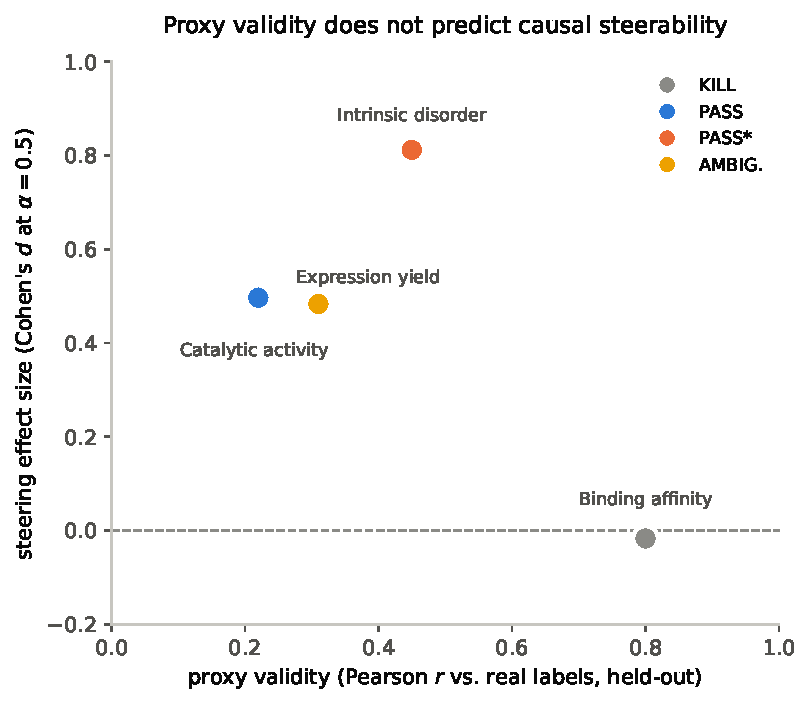
\includegraphics[width=0.68\linewidth]{figures/fig2_proxy_vs_effect.pdf}
\caption{The four runnable targets, plotted as explanatory validity
(proxy Pearson $r$ against real labels) against causal steering effect
size (Cohen's $d$ at $\alpha=0.5$). The most trustworthy explanation
(binding affinity, $r=0.80$) yields the least causally useful
intervention; a far weaker explanation ($r=0.22$, catalytic activity)
yields one of the two most causally effective interventions.}
\label{fig:proxy-vs-effect}
\end{figure}

\paragraph{Binding affinity.} Using a ProteinGym deep-mutational-scanning
assay of KRAS binding to a DARPin binder, we build a proxy from
per-position mutational-sensitivity weights learned on the training
split. This is the most rigorously validated explanation in our study:
$r=0.80$ held-out. A weight-shuffle null of $r=-0.001$ rules out a
generic rather than position-specific signal. The proxy also generalizes
to held-out positions, with $r=0.54$ on positions never seen during
weight fitting, and from single to double mutants, with $r=0.70$. The
causal intervention built from this
explanation is a flat, unambiguous null at every tested strength, with
zero degenerate sequences. This rules out generation collapse as an
alternative account. A plausible mechanistic reason
(\S\ref{sec:cases}): this dataset's vector-building groups are
single-backbone point mutants, giving the difference-of-means
construction very little raw compositional signal to act on, independent
of whether the underlying explanation is valid.

\paragraph{Catalytic activity.} A glycine-minus-arginine compositional
proxy on DLKcat (cross-protein enzyme turnover data), the weakest
explanation of the four runnable targets ($r=0.22$), matching the
published activity-stability tradeoff in enzymology. This produces a
clean, monotonic causal effect (Figure~\ref{fig:dose-response}, left),
significant at every safe-range $\alpha$, surviving residue-exclusion,
and replicated identically across three independent seeds. It is the one
target in our sweep with fully unanimous seed robustness despite the
weakest explanatory grounding.

\subsection{Intrinsic disorder: seed-sensitivity in a robustness criterion}
\label{sec:disorder-detail}

A proxy from the published TOP-IDP disorder-propensity scale
\citep{campen2008topidp} validates at $r=0.45$ (the strongest explanation
in our sweep), confirmed at the per-residue level (AUC $0.71$ via a
sliding window against real per-residue labels). In this case,
explanatory validity and evaluation rigor are both high. The causal
effect is significant and monotonically dose-responsive on all three
independent seeds (Figure~\ref{fig:dose-response}, right). However, the
residue-exclusion robustness check is analogous to a faithfulness check
on an explanation method. It passes on 2 of 3 seeds (36--42\% of
effect magnitude retained, CI excludes zero) and fails on the third (10\%
retained, CI crosses zero, Figure~\ref{fig:seed-robustness}). The causal
effect's existence and direction are seed-stable; the specific robustness
criterion is not, uniformly.

\begin{figure}[t]
\centering
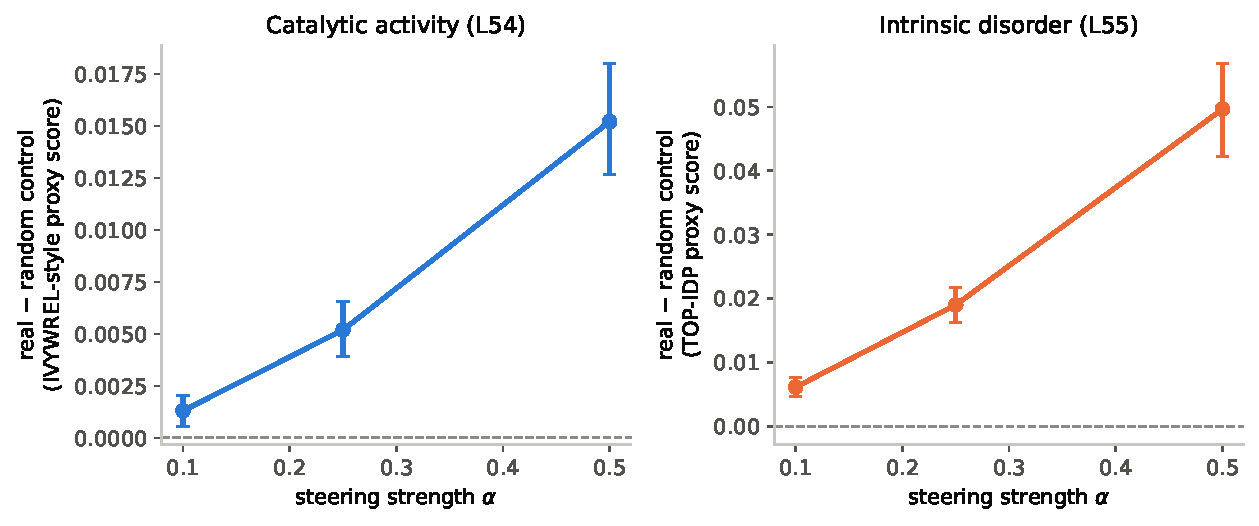
\includegraphics[width=\linewidth]{figures/fig1_dose_response.pdf}
\caption{Dose-response for the two targets passing criterion 2. Both
show a clean, monotonic increase with 95\% bootstrap CIs bounded away
from zero at every point.}
\label{fig:dose-response}
\end{figure}

\begin{figure}[t]
\centering
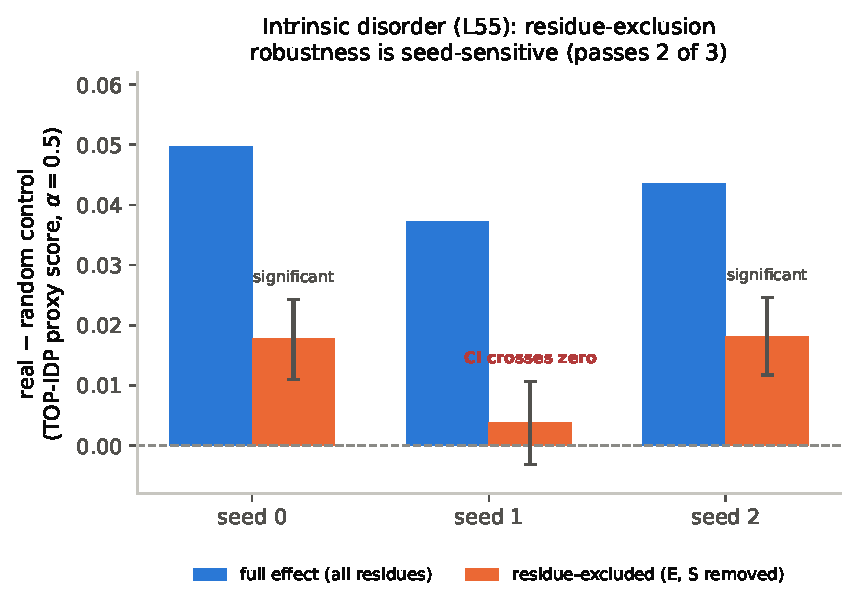
\includegraphics[width=0.7\linewidth]{figures/fig3_seed_robustness.pdf}
\caption{The intrinsic-disorder target's causal effect (blue) and the
same effect after the two dominant substituted residues are excluded
(orange, 95\% bootstrap CIs), across three independent seeds. The
underlying causal effect is stable across all three; the
residue-exclusion faithfulness check is significant on seeds 0 and 2 but
its CI crosses zero on seed 1. The causal effect is unchanged, but the
robustness criterion produces three different verdicts.}
\label{fig:seed-robustness}
\end{figure}

\paragraph{Immunogenicity.} We evaluate candidate explanatory proxies
across four tiers of increasing fidelity to the real target. Proxies
predictive on a surrogate binding-affinity tier ($r=0.37$--$0.43$)
collapse to near-chance on the real T-cell-response endpoint
($r\leq0.10$). A full-length-antigen proxy reaches $r=0.38$, but organism
identity alone explains 58\% of the apparent signal. The same proxy's
correlation flips to $-0.32$ once organism identity is held out of
cross-validation. This is a direct example of an apparently grounded
explanation that tracks an unrelated confound. No proxy survives
criterion 4, so no causal steering run was performed.

\paragraph{Expression yield.} A net-charge-deviation proxy validates at
$r=0.31$--$0.34$ and produces a significant, dose-responsive causal effect
that collapses under residue-exclusion. The explanation-validity check
passes, but the faithfulness check fails.

\section{Grounding an Ambiguous Result: A Vector-Geometry Diagnostic}
\label{sec:cases}

Rather than discarding the expression-yield result as unexplained noise,
we compute cosine similarity between its steering vector and every other
target's, layer by layer. We find substantial overlap with the
intrinsic-disorder target's vector: $+0.38$ on the full 33-layer
concatenation, rising to $+0.56$--$0.67$ at the three deepest layers. This
is consistent with the independently documented biology because
disordered protein regions are known to reduce solubility and expression
yield. It also grounds the result causally: expression yield's apparent effect is
best understood as a partial, noisier echo of disorder's already-validated
direction, filtered through a proxy more prone to compositional collapse,
not independent evidence of a sixth causally steerable property. This
diagnostic (compare a new intervention's direction against every other
validated direction in the same study) is a cheap, generalizable
faithfulness check for any study running multiple related causal
interventions.

\paragraph{A caught faithfulness-evaluation artifact.} As a mechanistic
follow-up on thermostability, we tested whether restricting steering to
the 5 layers previously identified as causally necessary preserves the
effect of steering all 33. A first evaluation selected its
best-performing $\alpha$ from the full tested range, including
$\alpha\geq1.0$, and concluded the 5-layer subset matched or exceeded the
full intervention. This was an artifact of the evaluation, not a real
result. At that $\alpha$, the 33-layer intervention had already fully
collapsed into degenerate output, leaving zero non-degenerate evaluation
sequences. The 5-layer subset had not yet collapsed. This evaluation
problem is directly analogous to comparing two explanation methods at
operating points where one has already failed.
Restricting the comparison to a range where neither arm has collapsed and
rerunning end to end gives the honest result: the 5-layer subset produces
a real, residue-robust effect, retaining only 43--59\% of the full effect
size.

The binding-affinity mechanistic account (\S\ref{sec:sweep}) is likewise
grounded, not asserted. The mean per-residue compositional distance
between this target's low/high vector-building groups is $0.003$, versus
$0.02$--$0.05$ for the three cross-protein targets in our sweep. This
provides a measurable reason that the causal construction had little
signal to use, independent of the explanation's own validity.

\section{Related Work}

\citet{huang2025steering} introduce difference-of-means activation
steering for protein language models and validate it causally on
thermostability; we extend their intervention to five new properties
under a pre-registered protocol and test, to our knowledge for the first
time, whether explanatory (proxy) validity predicts causal success across
multiple unrelated properties. \citet{vig2021bertology} identify the
attention head we redo as a genuine causal ablation test, extended here
to a full 480-head sweep with zero correlational information in the
ranking. \citet{adams2025mechanistic} train sparse autoencoders on
ESM-2's residual stream and use a purely correlational, post-hoc linear
probe to show that known determinants of thermostability and subcellular
localization are identifiable in SAE
feature space; their one steering experiment is a coherence check (does
steering change fewer residues than a random direction), not a validation
against a real causal ground truth, and their discussion states plainly
that ``investigating how to steer the model in useful ways remains an
open direction for future work.'' Our work answers a version of that
question directly: whether an interpretability method's correlational
validity, evaluated rigorously by the field's own standards, predicts the
causal usefulness of an intervention built on it.

\section{Discussion}

\paragraph{What ``causal'' means here.} Every result in this paper is
causal about the model's activation space. It reflects a real
intervention on the forward pass, evaluated against a matched-norm
random-direction control and a residue-exclusion faithfulness check on
generated sequences. It is not validated against a real biological
assay. A PASS means ``causally steers a validated compositional
explanation,'' not ``causally engineers the underlying biological
property.'' This distinction matters when claiming that an
interpretability method's causal usefulness has been established.

\paragraph{Limitations.} All experiments use one foundation model,
ESM2-650M, at one scale. We did not test whether the findings hold at
other scales, so it remains unclear whether the mismatch between
explanatory validity and causal effect is specific to this model or more
general. All proxies are compositional heuristics chosen for
interpretability and speed rather than learned attribution methods. A
stronger explanation method might show a different relationship to
causal effect.

Each target's final proxy was selected as the best of several candidates
scored on the same held-out split used for its reported validation $r$.
We did not use a separate select/test split. This choice inflates every
reported proxy-$r$, so the absolute values should be read as upper bounds.
It does not obviously overturn the ordinal mismatch on which the central
claim rests. We also ran many significance tests without a
multiple-comparisons correction. Requiring multi-alpha and multi-seed
agreement for any PASS partially mitigates this issue, but individual
borderline criteria remain close to the noise floor. We checked seed
robustness for only two of five targets and did not run structural or
functional plausibility checks on generated sequences. A PASS therefore
does not rule out physically or biologically implausible proteins.

\section{Conclusion}

Correlational validity does not predict causal effect when a downstream
intervention built on it is tested at two levels of the same foundation
model class. This holds both for an attention head's alignment with a
known biological signal and for a scoring proxy's correlation with real
experimental labels. For interpretability methods intended to
guide scientific discovery or trustworthy intervention in biology, this
argues for validating explanations against the causal interventions they
are meant to support, not treating correlational or attribution-based
salience as self-certifying evidence of causal usefulness.

\bibliographystyle{plainnat}
\bibliography{reference}

\end{document}
